\documentclass{article}
\usepackage[a4paper, total={6in, 8in}]{geometry}
\usepackage{graphicx}
\usepackage{url}
\usepackage{natbib}
\usepackage{todonotes}
\usepackage{booktabs}
\usepackage{lineno}
\usepackage{color}
%\usepackage{auto-pst-pdf}
\usepackage[colaction]{multicol}
\usepackage{caption}
\usepackage{svg}
\usepackage{authblk}
\usepackage{standalone}
\usepackage[section]{placeins}

\usepackage{xr}
\externaldocument{main}

\makeatletter
\renewcommand{\maketitle}{\bgroup\setlength{\parindent}{0pt}
	\begin{flushleft}
		
		{\huge\textbf{\@title}}
		
		\bigskip
		
		{\large\textbf{\@author}}
		
		\bigskip
		
		{\large{ \@date}}
		
	\end{flushleft}\egroup
}
\makeatother


\begin{document}
	% Title
	\title{A Topic Model of Climate Change Literature}
	\title{Words, words, words: Mapping the Matter of Climate Change Literature}
	\title{A Topography of Climate Change Research}
	
\author[1,2]{Max Callaghan*}
\author[1,2]{Jan Minx}
\author[2]{Piers M. Forster}

\affil[1]{Mercator Research Institute on Global Commons and Climate Change, Torgauer Straße, 10829 Berlin, Germany}
\affil[2]{Priestley International Centre for Climate, University of Leeds, Leeds LS2 9JT, United Kingdom}
	\maketitle
	\begin{linenumbers}
		

		
		
		\section*{Methods}
		
					\setcounter{table}{0}
		\renewcommand\thetable{SI.\arabic{table}}  
		
		\subsection*{Data}
		
		This study reproduces the query developed by \citep{Grieneisen2011}, which is carried out on the Web of Science core collection. We downloaded the results of the query on March 19, 2019. Though not exhaustive, the Web of Science gives a good coverage of the literature in major peer-reviewed journals. The Web of Science data gives us a disciplinary classification (based on the journal) and publication year, among other metadata, for each document.	Each document is assigned to an assessment period according to the timeline shown in table 1.
		
		We also tested the query documented in \cite{Haunschild2016}, by checking a random sample of documents exclusive to it. We found that the majority of additional documents were not relevant, and decided to use only the query from \cite{Grieneisen2011}.
		
		We use the references scraped from IPCC assessment reports from \citep{Minx2017l}, and attempt to match these with the results from the Web of Science. We use doc2vec similarity scores \cite{Le2014} to identify the 500 most similar titles for each reference, and count the document as a match if the jaccard similarity score of the two word shingles of the reference title and the document title is greater than 0.5 \cite{Khabsa2014}. Table \ref{ipcc-matching} shows the percentage of IPCC citations matched in each working group for each assessment report. This is significantly lower in earlier periods, as data coverage and quality of citation databases is lower for earlier periods. Matching in WG III is also lower, suggesting a greater share of non-peer review literature, or literature not directly mentioning climate change, but related to its mitigation (for example on energy policy).
		
		We analysed by hand a sample of 100 IPCC references which could not be matched and found that 46\% of these references were not in the Web of Science at all, 53\% were in the Web of Science but not in our query, and 1 document was in our query but had mistakenly been identified as not being so. This was due a different version of the title appearing in the IPCC citation and the Web of Science record. 
		
		
		\begin{table}[htp]
			\begin{center}
				\begin{tabular}{lrrrrr}
\toprule
AR &  1 &   2 &   3 &   4 &   5 \\
WG &    &     &     &     &     \\
\midrule
1  & 8\% & 25\% & 37\% & 47\% & 58\% \\
2  & 6\% & 12\% & 30\% & 38\% & 47\% \\
3  & 3\% &  9\% & 15\% & 22\% & 35\% \\
\bottomrule
\end{tabular}

				\caption{The proportion of citations in each report that could be matched with a document in our query from the Web of Science}
				\label{ipcc-matching}
			\end{center}
		\end{table}
		
		
		\subsection*{Pre-processing}
		
		Data quality in earlier Web of Science results is poorer, and some documents have missing abstracts. In the quantification of the size of the literature and its vocabulary in table \ref{tab}, titles are substituted for abstracts where they are not available.  The words of the documents are lemmatized, replacing different forms of the same word (i.e. word/words) with a single instance. Commonly occurring words, or ``stopwords'' are removed, as are all words shorter than 3 characters, and all words containing only punctuation or numbers.
		
		The documents are transformed into a document-term matrix, where each row represents a document, and each column represents a unique word.  Each cell contains the number of that column's terms in that document. Only terms which occur more than once are considered.
		
		For the calculation of the topic model, documents with missing abstracts are ignored, and the document term matrix is transformed into a document
		frequency-inverse document frequency (tf-idf) matrix, where scores are scaled according to the frequency of their occurrence in the corpus. This gives more weight to terms which appear in few documents, and less weight to those which appear in many.
		
		\begin{equation}
		tf(t,d) = f_{t,d} \mathrm{,}\quad idf(t,D) = \log\frac{N}{|\{d \in D:t \in d\}|}
		\end{equation} 
		
		\subsection*{Topic Model}
		
		We use non-negative Matrix Factorisation (NMF) \cite{Lee1999}, an approach to topic modelling which factorises the term-frequency-inverse document frequency matrix \( V \) into the matrices \(W\), the topic-term matrix, and \( H \) the document-topic matrix, whose product approximates \(V\):
		
		\begin{equation}
		V_{i\mu} \approx (WH)_{i\mu} = \sum_{a=1}^{r}W_{ia}H_{a\mu}
		\end{equation}
		
		As demonstrated in Figure \ref{doc-topic}, each topic is represented as a set of word scores, and each document a set of topic scores. The combination of the two approach the word scores in the document. For clarity in the figure, these are shown as simple counts, but in the model these are scaled according to each term's frequency within the corpus as explained above.
		
		Topics are calculated using the scikitlearn library \cite{Pedregosa2011}, and are saved in a database and topic visualisation system based on \cite{Chaney2012} \footnote{The system adds new functionality to \cite{Chaney2012} and combines it with a system for managing sets of documents and queries. The code and additional information is published online at \url{https://github.com/mcallaghan/tmv}}. 	
		
		\subsubsection*{Model selection}
		
		Topic models are calculated for 70, 80, 90, 100, 110, 120, 130, 140 and 150 topics. The run with 150 topics was discarded as it contained a topic to which no terms or documents were assigned. The relative usefulness of each model was assessed subjectively by the authors, based on inspection of the online visualisation tool, and the spreadsheet \textbf{topic\_comparison.xlsx} accompanying the supporting information. The spreadsheet shows each set of topics in adjacent columns. Topics from each model are placed next to the topics with the largest number of each topic's 10 highest scoring words in common. This helps authors to find an appropriate level of granularity for the analysis. Statistical methods for the selection of topic model parameters are available but they do not necessarily align with human perceptions of topic model quality \cite{Chang2009}. We make a judgement based on subjective criteria, but for transparency publish the results of the analysis for different numbers of topics in figure \ref{top-rep-ks}. The main conclusions drawn about the rapid growth and under-representation of solutions-relevant topics are stable across models.
		
		
		\subsubsection*{Topic assignment to working groups}
		\label{topic-wg}
		A topic's score for each working group is calculated by summing the document-topic scores for all documents cited by that working group. We call the topic's primary working group that working group for which the above sum is the highest, but in some cases, where there are very few IPCC citations of documents related to a topic this can be misleading . For example, the word ``capacity" is relevant to the adsorption topic, so documents talking about adaptive capacity receive a low score for the topic. Because only very few documents highly relevant to the topic (in that they talk about adsorption or adsorptive capacity) are cited by the IPCC, and many of the weakly relevant documents are cited by the IPCC, the sum of the topic scores of the weakly relevant documents outweighs the sum of the topic scores of the strongly relevant documents, meaning that the topic is mistakenly assigned to working group II when it is more properly relevant to working group III. We point out that topics are in any case mixtures of documents cited by different working groups, and stress that the colouring of the topics by working group is merely illustrative.
		
		
		\subsubsection*{Topic Representation and Newness}
		
		To calculate topic representation in IPCC reports we divide each topic's share in the subsample of documents cited by IPCC reports by its share in the whole corpus (excluding documents published after the last assessment report). Disciplinary representation is calculated in the same way.
		
		We calculate a topic's total score as the sum of document-topic scores. A topic's window score is the sum of document-topic scores considering only documents in the given time window. To represent a topic's newness, we multiply each assessment period number by the share of it's total score occurring in that window, and take the mean of these scores. A topic in which 100\% of documents which make it up occurred in assessment period 1 (6) would thereby receive a score of 1 (6), while a topic evenly distributed across all assessment periods would receive a score of 3.5.
		
		
		\subsubsection*{Disciplinary Entropy}
		
		Disciplinary Entropy inverts the measurement of a conference's topical diversity suggested in \cite{Hall2008}, by measuring a topic \(z\)'s entropy \(H\), where 
		
		\begin{equation}
		H(f|z) = -\sum_{i=1}^K \hat{p}(f|z) \log \hat{p}(f|z) 
		\end{equation}
		
		based on the empirical distribution of a field \(f\) in the documents \(d\) in each topic:
		
		\begin{equation}
		\hat{p}(f|z) = \sum_{d:z_d=z} \hat{p} (f|d) \hat{p} (d|z)
		\end{equation}
		
		It is an indication of the diversity of disciplines within the set of documents related to a topic. 
		
		\subsubsection*{Topic Map}
		The topic model gives us the location of each document in a 140 dimensional topic space, with each dimension corresponding to a that document's \textit{topic-ness} in a given topic. t-Distributed Stochastic Neighbour Embedding (t-SNE) is a dimensionality reduction technique which we use to represent each document's topic scores in 2 dimensions \cite{vandermaaten2008}. Documents are placed on the map such that documents with similar combinations of topics are close together.
		

		
		
		\subsection*{Glossary}
		
		\noindent\textbf{co2:} Carbon Dioxide
		
		\noindent\textbf{ncep:} National Centers for Environmental Protection
		
		\noindent\textbf{fco:} Fugacity of Carbon Dioxide
		
		\noindent\textbf{pfc:} Perflourocompound
		
		\noindent\textbf{otcs:} Open Top Chambers
		
		\noindent\textbf{dtr:} Diurnal Temperature Range
		
		\noindent\textbf{sres:} Special Report on Emissions Scenarios (200)
		
		\noindent\textbf{petm:} Paleocene Eocene Thermal Maximum
		
		\noindent\textbf{amf:}  Arbuscular Mycorrhizal Fungal
		
		\noindent\textbf{sf5cf3:} trifluoromethyl sulfur pentafluoride (A Potent Greenhouse Gas Identified in the Atmosphere, 2000)
		
		\noindent\textbf{clc:} Chemical Looping Combustion
		
		\noindent\textbf{cwd:} Coarse woody debris
		
		\noindent\textbf{etm:} Enhanced Thematic Mapper (NASA satellite sensor)
		
		\noindent\textbf{cmip5:} Coupled Model Intercomparison Project 5 (Starting 2008)
		
		\noindent\textbf{cmip3:} Coupled Model Intercomparison Project phase 3 (first published 2007 \cite{Meehl2007})
		
		\noindent\textbf{mofs:} metal-organic frameworks (for CO2 storage)
		
		\noindent\textbf{sdm:} statistical-dynamical model
		
		\noindent\textbf{mmms:} Mixed Matrix Membranes (for CO2 capture)
		
		\noindent\textbf{cop21:} 21st Conference of Parties (Paris 2015) 
		
		\noindent\textbf{c3n4:} Carbon nitride (a synthetic nanomaterial used for hydrogen production)
		
		\noindent\textbf{sdg:} Sustainable Development Goals
		
		\noindent\textbf{(i)ndc:} (Intended) Nationally Determined Contributions
		
		
	\end{linenumbers}
	
	\linespread{1}
	

	
	\section*{Supplementary Figures}
	
			\setcounter{figure}{0}
	\renewcommand\thefigure{SI.\arabic{figure}}  
	
	\begin{figure}
		\begin{center}
			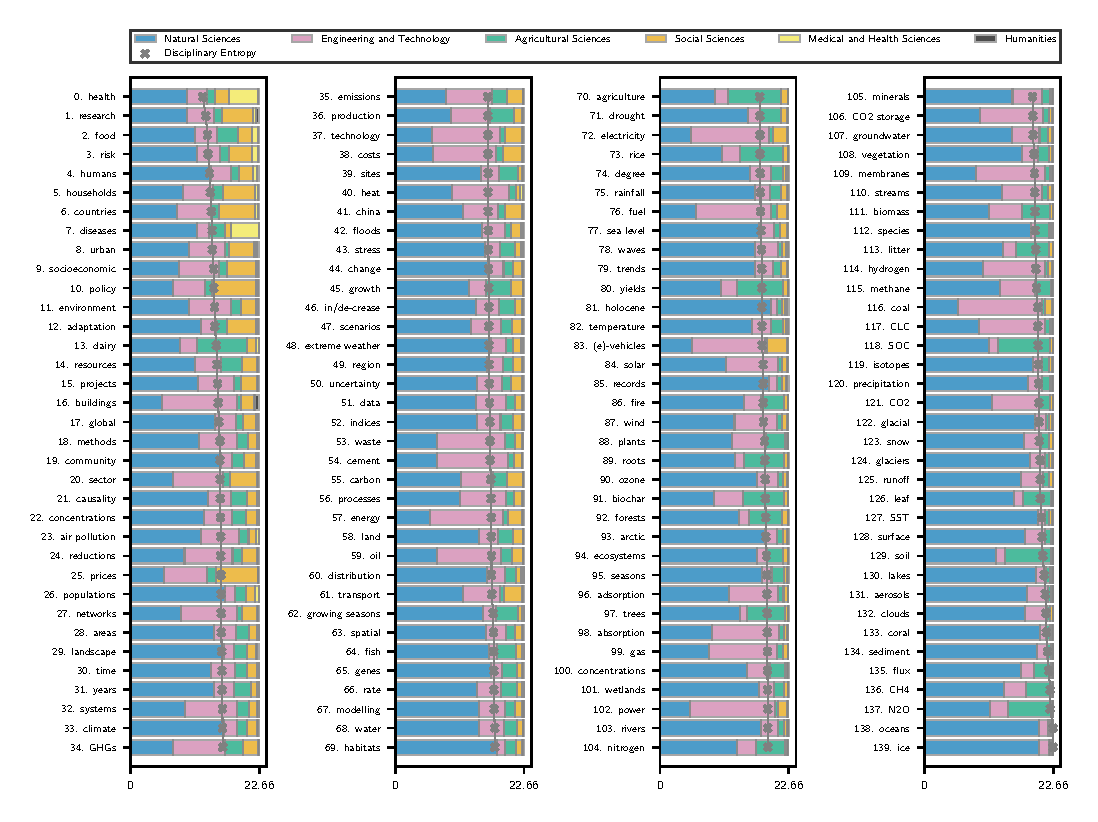
\includegraphics[width=1\linewidth]{../plots_pub/topic_oecd_entropy.pdf}
			\caption{Disciplinary Entropy of Topics. Coloured bars show the proportion of each topic made up of papers from each disciplinary category. Crosses show the Disciplinary Entropy of each topic (see methods for details).}
			\label{dis-entropy}
		\end{center}
	\end{figure}	
	
	
	
	\begin{figure}
		\begin{center}
			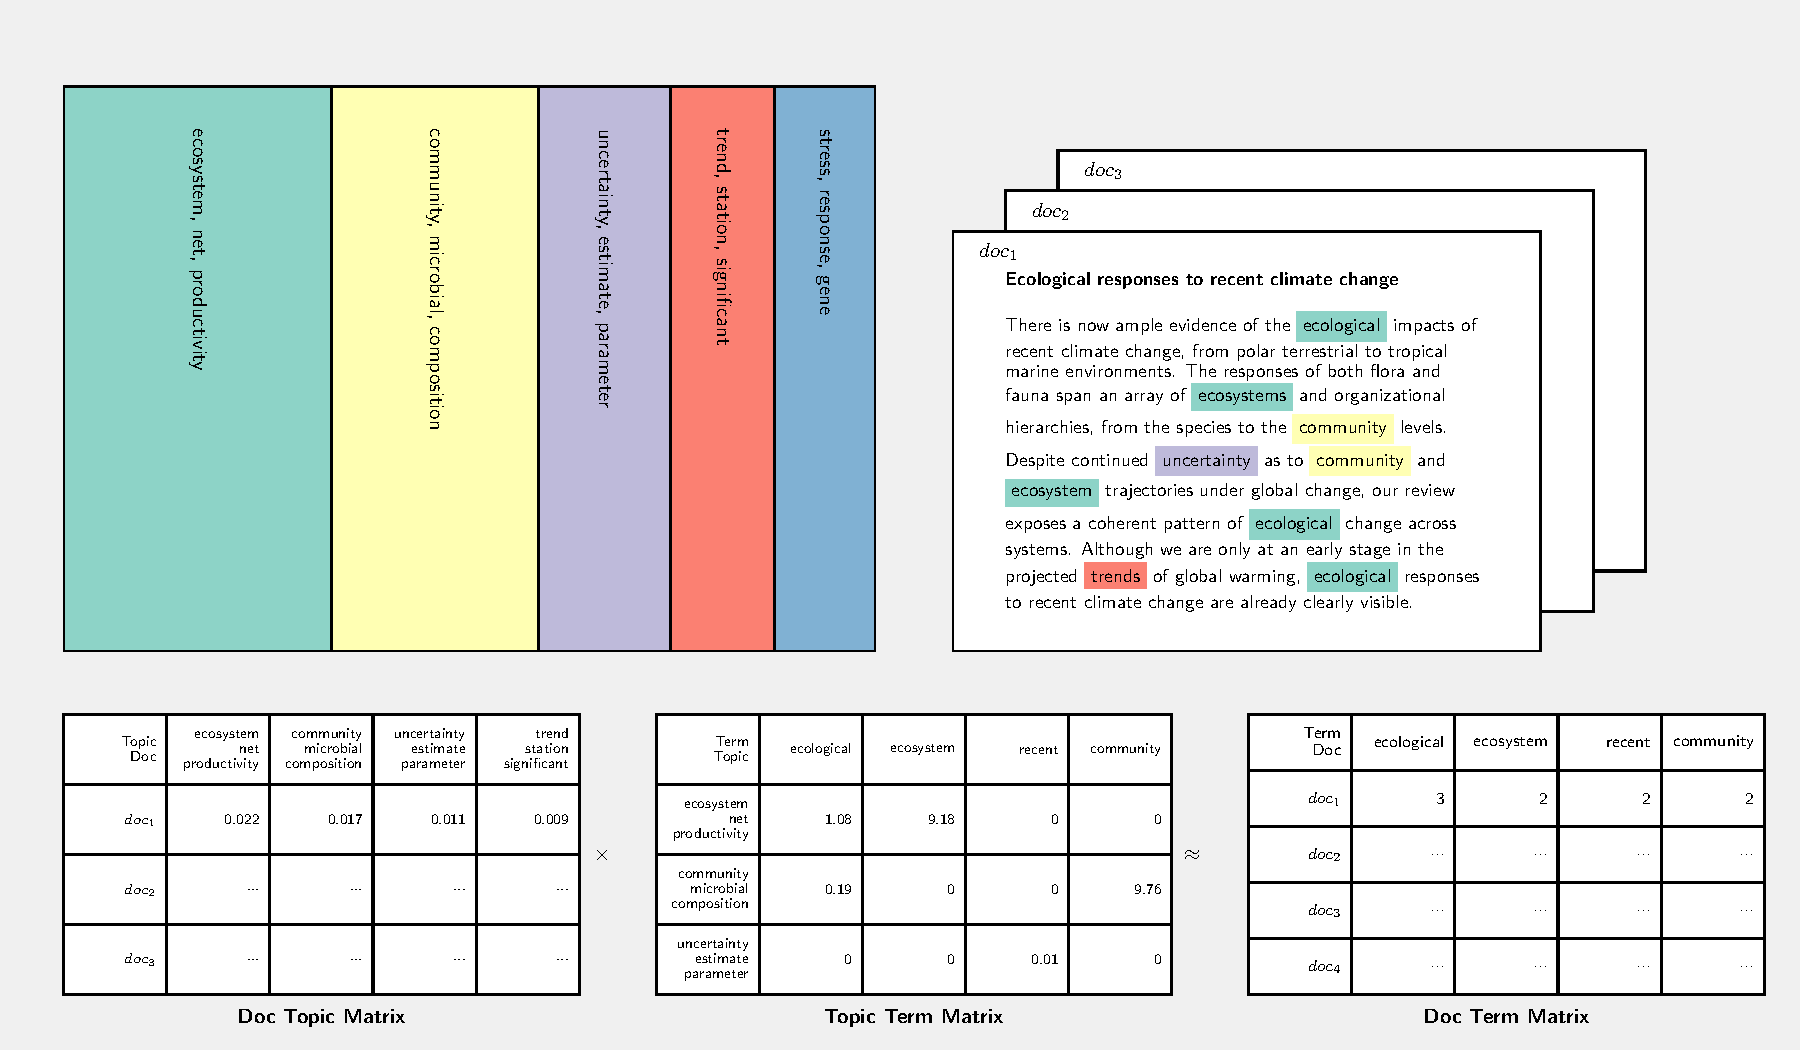
\includegraphics[width=1\linewidth]{../plots_pub/single_doc_3_536594_1861.pdf}
			\caption{Topic make up of a single document. The Doc Term Matrix shows the number of occurrences of each term in the document. The Topic Term Matrix shows the topic score of each term-topic combination. The Doc Topic Matrix shows the document-topic score for each topic. This topic makeup of the document shown is illustrated by the bars in the top left. Words highly associated with each topic that occur in the document are highlighted. All values are real, although the doc-term matrix is scaled by the inverse-document frequency before being used in the model.}
			\label{doc-topic}
		\end{center}
	\end{figure}
	
	\begin{figure}
		\begin{center}
			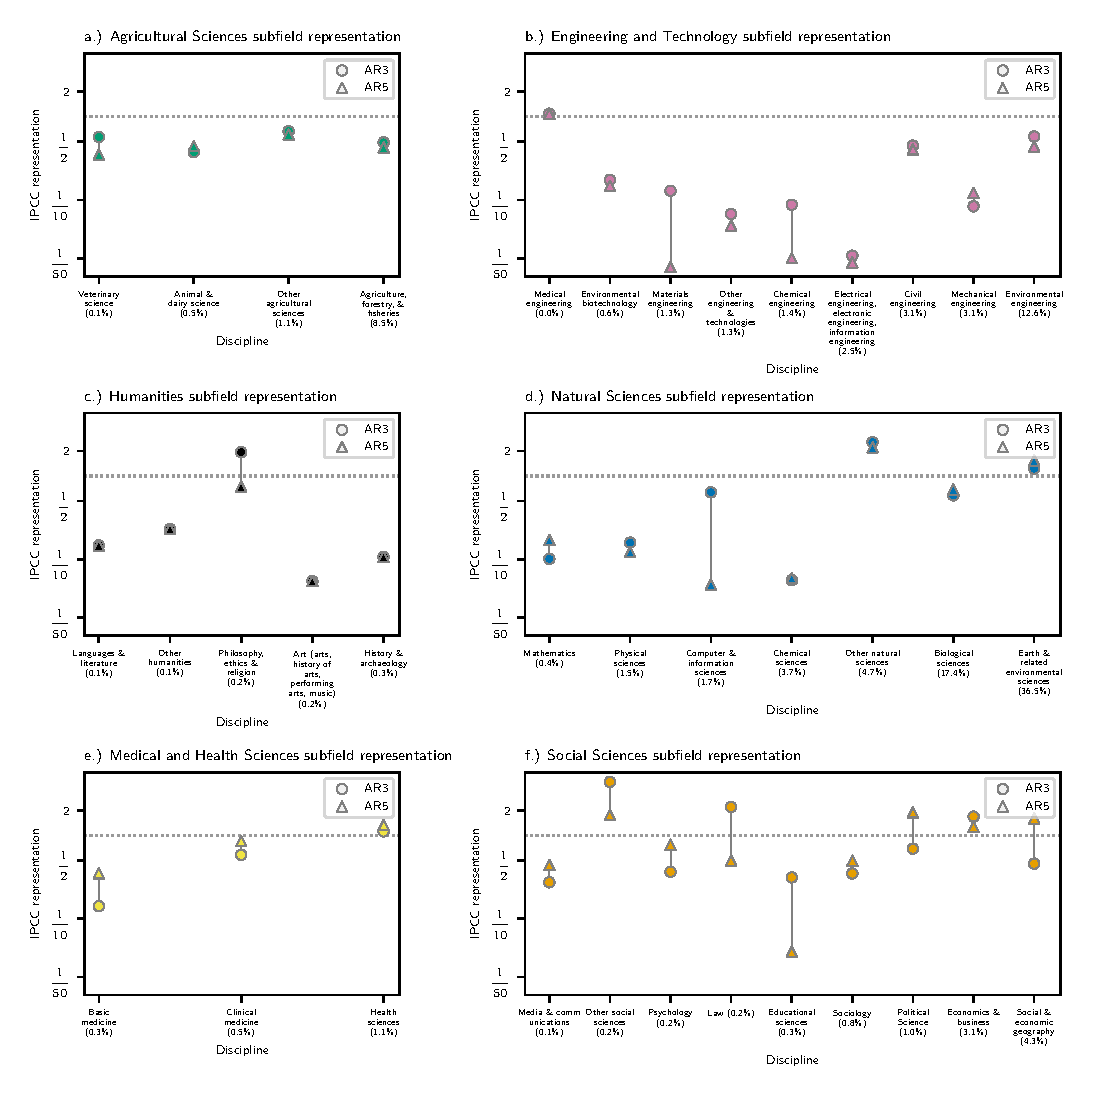
\includegraphics[width=1\linewidth]{../plots_pub/ipcc_rep_wcs_simplified.pdf}
			\caption{IPCC Representation by subfield. Representation is the share of the subset of documents being cited by the IPCC divided by the share of the subset in the whole literature. We plot on a log scale so that 0.5 is equally distant to 1 as 2; plot labels show real values.}
			\label{subfield}
		\end{center}
	\end{figure}
	
	\begin{figure}
		\begin{center}
			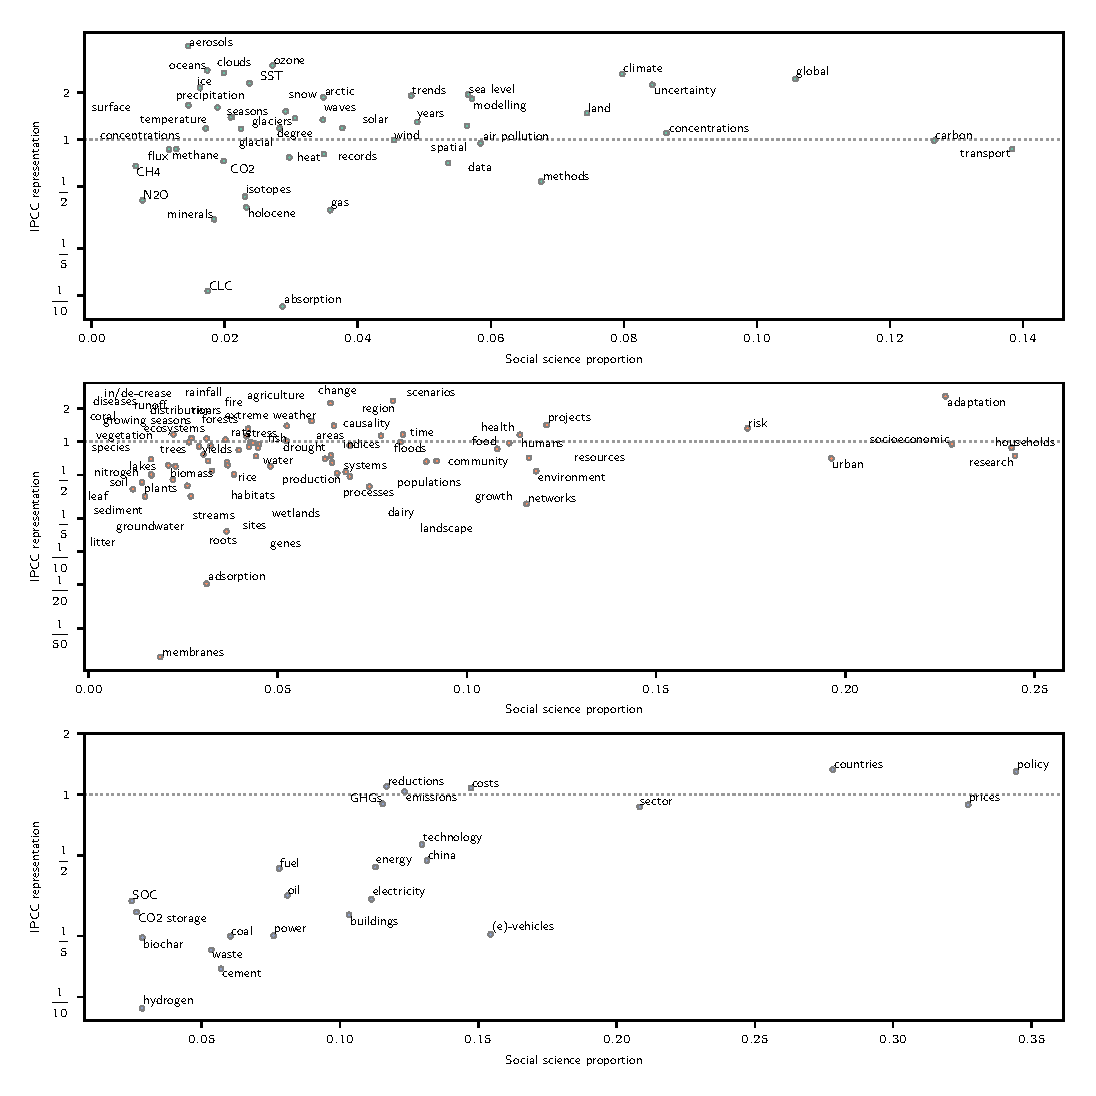
\includegraphics[width=1\linewidth]{../plots_pub/wgs_socsci.pdf}
			\caption{SI Social science \& representation in topics across working groups. Representation is the share of the subset of documents being cited by the IPCC divided by the share of the subset in the whole literature. Social science proportion shows the proportion of the total document-topic score coming from documents in the social sciences.}
			\label{socsci-wgs}
		\end{center}
	\end{figure}
	
	\begin{figure}
		\begin{center}
			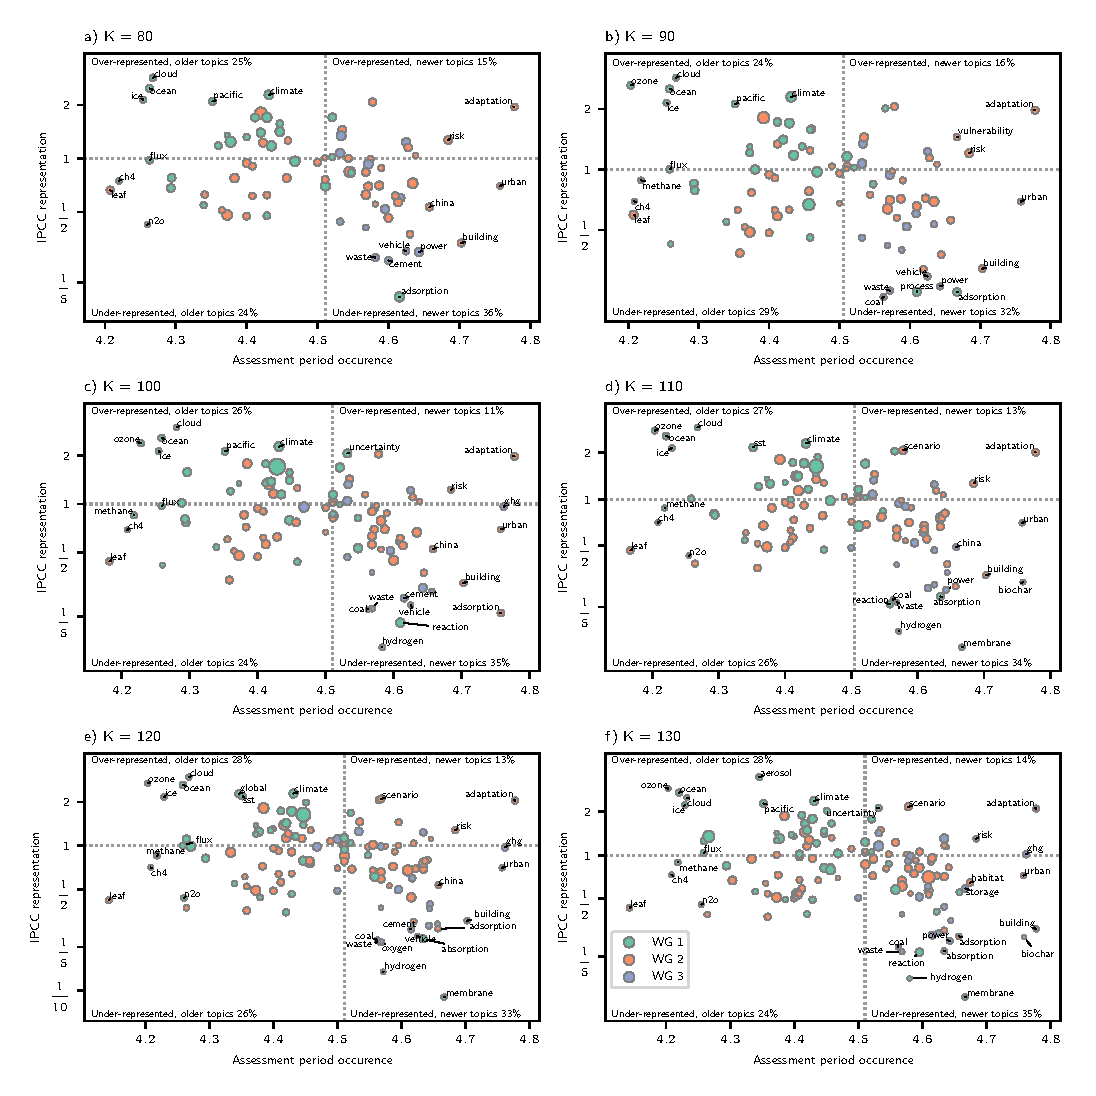
\includegraphics[width=1\linewidth]{../plots_pub/topic_rep_ks.pdf}
			\caption{Topic representation over different values of K (number of topics). Topics in the upper or lower 6.66th percentile of either dimension are labelled. Representation is the share of the subset of documents being cited by the IPCC divided by the share of the subset in the whole literature. Assessment period occurrence refers to the center of a topic's distribution across assessment periods (see methods for further details).}
			\label{top-rep-ks}
		\end{center}
	\end{figure}
	
	\section*{Data Availability}
	
	Three datasets from this study are available at \url{https://doi.org/10.6084/m9.figshare.9009665}
	
	\medskip\noindent
	\texttt{docs.csv} contains a list of the documents considered in this study, along with basic metadata and their position on the map. For copyright reasons, the full metadata from Web of Science can not be published. To reproduce the analysis, it would be necessary to download the abstracts for the papers shown, either using the Web of Science IDs provided, or the query documented in \cite{Grieneisen2011}.
	
	\medskip\noindent
	\texttt{topics.csv} Contains a list of the topics, along with their features discussed in this paper. The top 10 words associated with each topic are also shown
	
	\medskip\noindent
	\texttt{doctopics.csv} Contains a list of document-topic scores, which can be cross-referenced with the document and topic ids in \texttt{docs.csv} and \texttt{topics.csv}.
	
	\medskip\noindent
	\texttt{topic\_comparison.xlsx} shows models with different numbers of topics. It was used to select the topic model used for analysis in this paper.
	
	\section*{Code Availability}
	
	The code used to produce this paper is available at https://github.com/mcallaghan/cc-topography
	
	
	\bibliography{Mendeley}
	\bibliographystyle{unsrt}
	
	
	
\end{document}